%{Cold Boxes Cryogenics}
\label{sec:fdsp-tc-cryocoldbox}


The  \coldbox{}es will be used to test the \dword{apa}s underground prior to installation.  
The cryogenics supporting the \coldbox{}es  must ensure their reliable and safe operation; to that end, it must
\begin{itemize}
\setlength\itemsep{1mm}
\setlength{\parsep}{1mm}
\setlength{\itemsep}{-5mm}
\item support three \coldbox{}es operating in parallel: %for testing dual \dword{apa}s: 
one in \cooldown mode, two either in steady-state or warm-up modes.
\item allow personnel in the cleanroom during all phases of the purge, \cooldown, operation, and warm-up modes. 
\item test the detector modules at near \dword{lar} temperature.
\item operate 24 hours a day.
\item allow remote operations.
\item be located in the vicinity of the \dword{tco}. Space is available on top of the cryogenic mezzanine on the roof of the cryostat.
\end{itemize}

It must operate in the following modes: %fulfill the following modes of operations:

\begin{itemize}
\setlength\itemsep{1mm}
\setlength{\parsep}{1mm}
\setlength{\itemsep}{-5mm}
\item \textbf{purge}: During this mode, air is removed from the system (\coldbox and cryogenic system) and replaced with dry nitrogen. The concentration of moisture is monitored, and when it no longer decreases, the \cooldown can commence.
\item \textbf{\cooldown}: Cold nitrogen is introduced into the system to cool the inside of the \coldbox and the \dword{apa} inside it. 
This should take 24 hours, during which time the temperature decreases from room temperature to about \SI{90}{K}. 
\item \textbf{steady-state operations}: After reaching approximately \SI{90}{K}, 
the detector is turned on and fully tested. 
This takes about 2 shifts.
\item \textbf{warm-up}: After completing the test, the system is
warmed up to room temperature over a period of 24 hours. 
\end{itemize}

\begin{dunetable}
[\Coldbox  cryogenics system parameters] %for specifications]
{lc}
{tab:table-cryo-coldboxes}
{Table of parameters for the \coldbox cryogenics system.}
Parameter & Value 
\\ \toprowrule
Dual \dword{apa} thermal mass &  1,600 kg\\ \colhline
Temperature uniformity & $+60$ K / $-0$ K \\ \colhline
Electronics load & 300 W \\ \colhline
\Coldbox insulation thickness &  0.3 m \\ \colhline
Target \cooldown temperature &  \SI{90}{K} \\ \colhline
Target \cooldown duration &  24 hr \\ \colhline
Target steady-state duration &  24 hr \\ \colhline
Target warm-up duration &  24 hr \\ \colhline
Maximum cooling power  &  \SI{13}{kW}  \\ \colhline 
Maximum liquid nitrogen consumption  &  \SI{300}{l/hr}  \\ \colhline 
\end{dunetable}

The evaporation of liquid nitrogen provides the cooling power for the system. Warm nitrogen and a heater provide the heating power. At peak consumption, the expected maximum heat load is \SI{8.5}{kW}. Assuming a 50\% margin on the refrigeration load, the cryogenics system requires \SI{13}{kW} of net cooling power at peak consumption, which equals about \SI{300}{l/hr} of evaporating liquid nitrogen.

Two layouts are currently under consideration: (1) a closed loop with mechanical refrigeration, in which liquid nitrogen is generated {\it in situ}, circulated, and the spent nitrogen recondensed before being put back into the system; and (2) open loop, in which liquid nitrogen is transported underground by means of portable dewars, circulated, and the spent nitrogen vented away. For the closed loop, we would need a mechanical refrigeration capable of supplying \SI{13}{kW} of cooling. For the open loop, it is possible to use a \SI{2000}{l} dewar, which is commercially available and transportable up and down the Ross Shaft inside the cage. To supply the required amount of nitrogen, four trips per day are needed.

The current versions of the closed loop and open loop systems are presented in Figures~\ref{fig:mechanical-refrigeration} and~\ref{fig:LN2}, respectively. 

\begin{dunefigure}[\Coldbox cryogenics support system based on mechanical refrigeration ]{fig:mechanical-refrigeration}
  {Layout of the cryogenics supporting the \dword{apa} test facility with mechanical refrigeration (closed loop).}
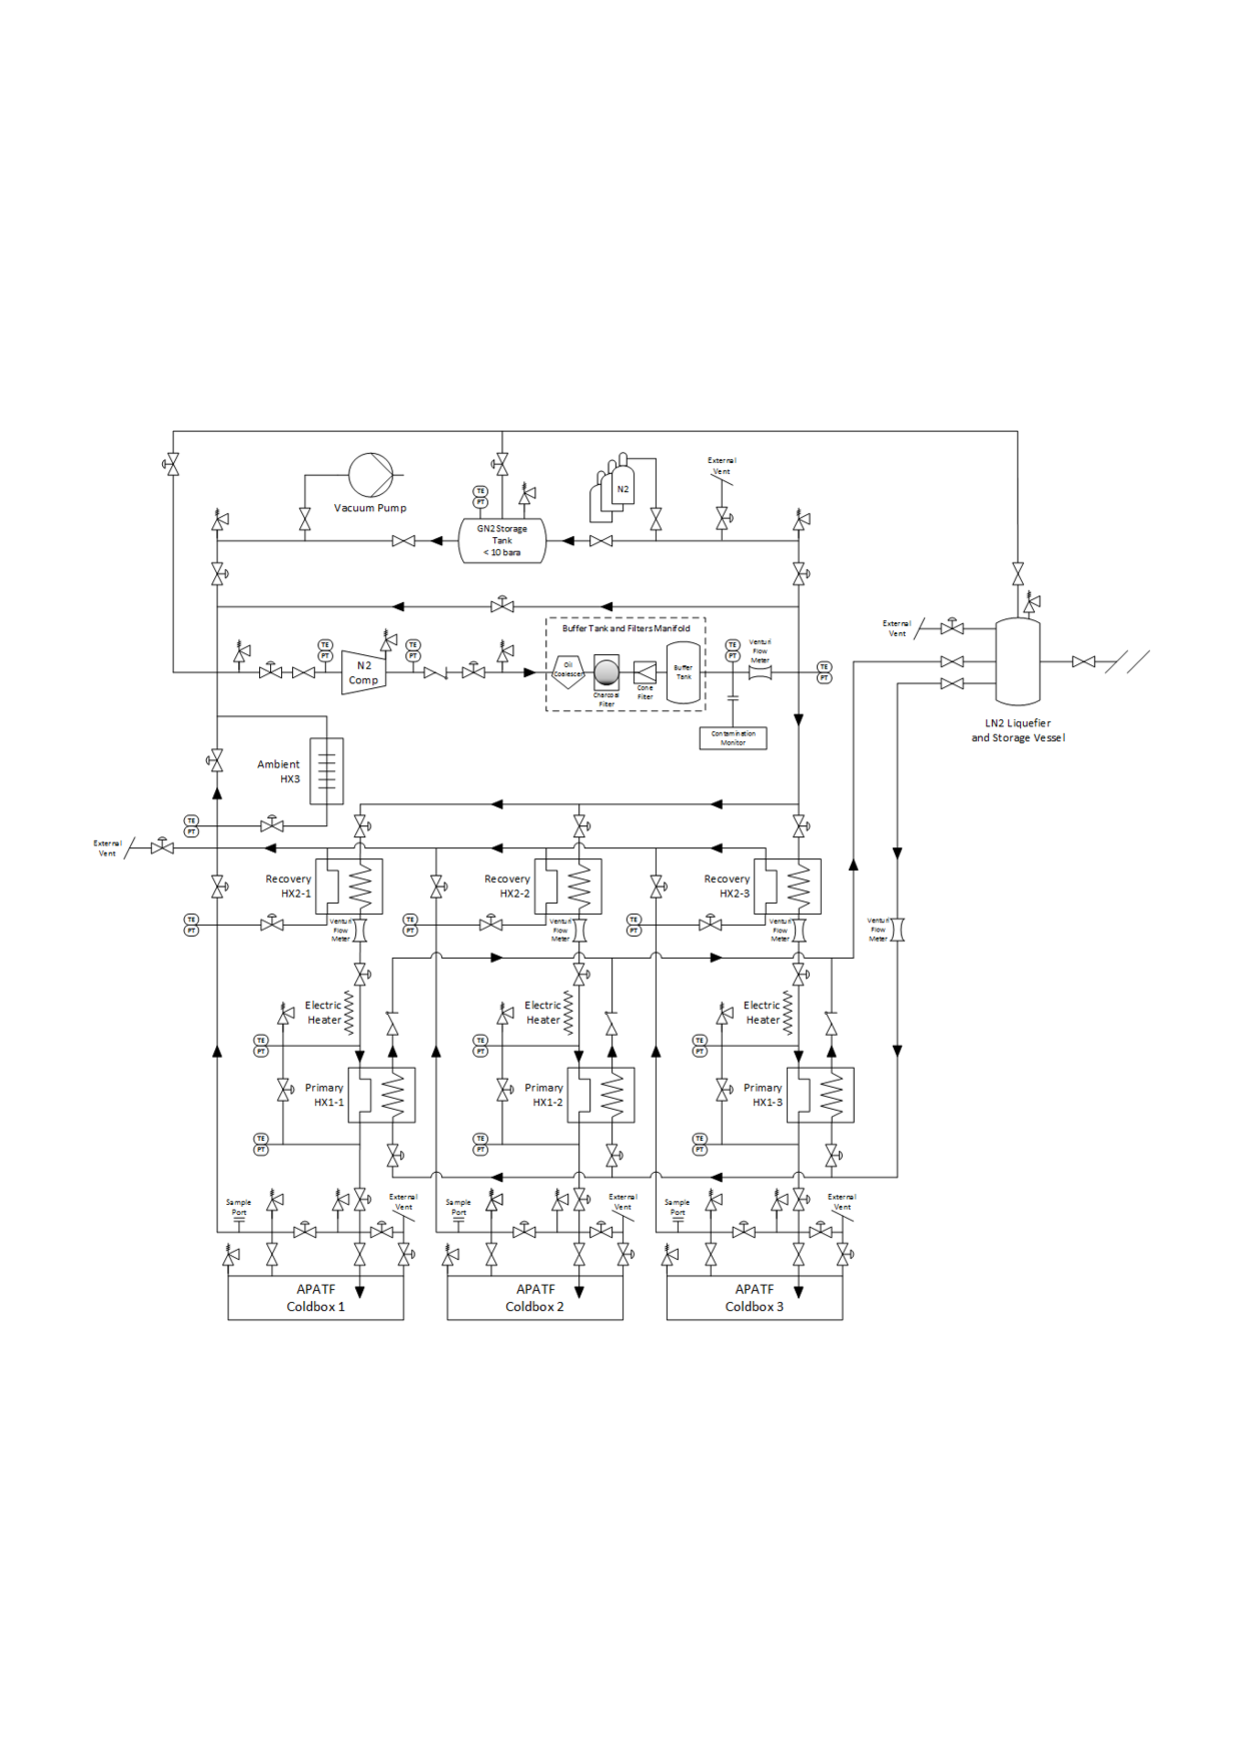
\includegraphics[width=.98\textwidth]{graphics/Cryo-cold-box-mechanical.pdf}
\end{dunefigure}

\begin{dunefigure}[\Coldbox cryogenics support system based on LN2 ]{fig:LN2}
  {Layout of the cryogenics supporting the \dword{apa} test facility with open loop refrigeration (open loop).}
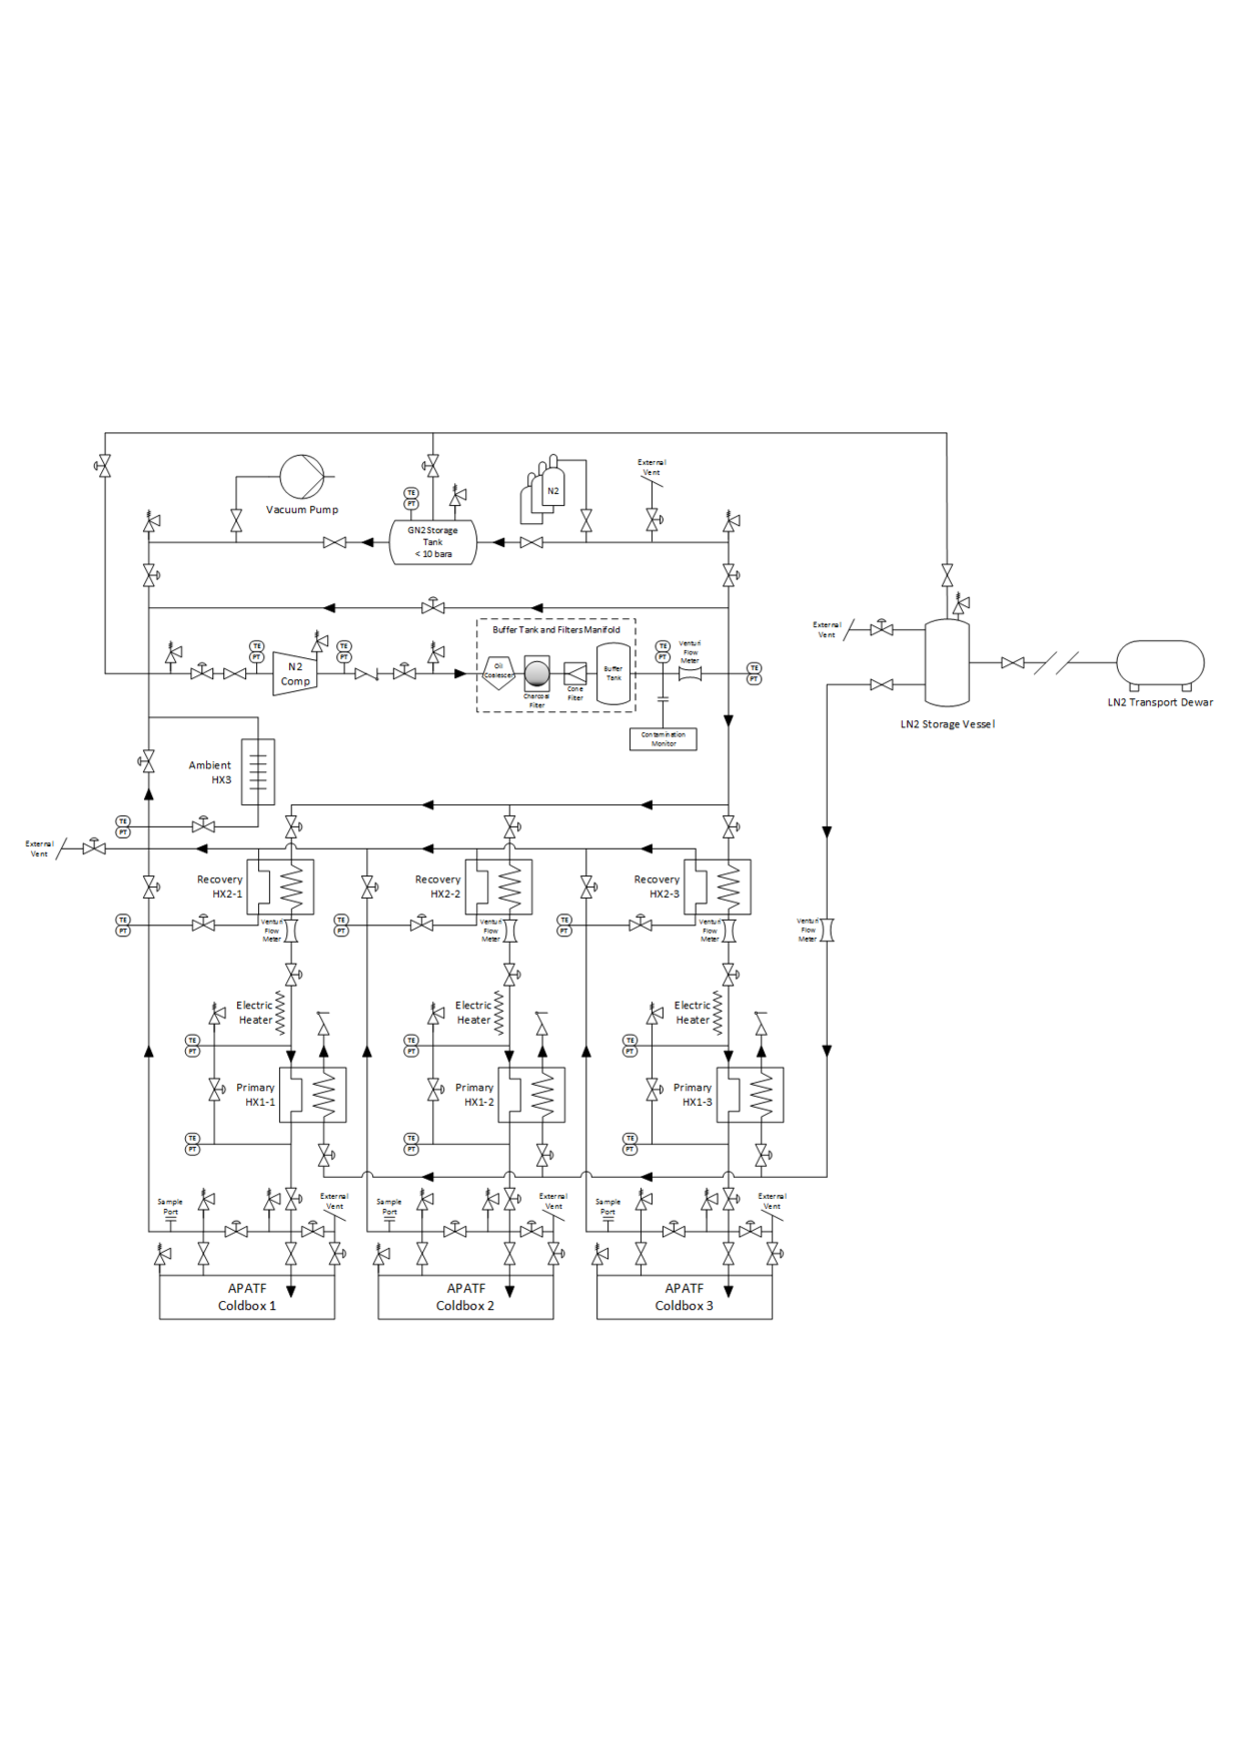
\includegraphics[width=.98\textwidth]{graphics/Cryo-cold-box-LN2.pdf}
\end{dunefigure}



%%%%%%%%%